\documentclass[nofootinbib,amssymb,amsmath]{revtex4}
\usepackage{mathtools}
\usepackage{amsthm}
\usepackage{algorithm}
\usepackage{algpseudocode}
\usepackage{lmodern}
\usepackage{graphicx}
\usepackage{color}

\newcommand{\RCS}{\texttt{ReCapSeg}}
\newcommand{\ACS}{\texttt{AllelicCapSeg}}

%Put an averaged random variable between brackets
\newcommand{\ave}[1]{\left\langle #1 \right\rangle}

\newtheorem{lemma}{Lemma}
\newtheorem{corollary}{Corollary}

\def\SL#1{{\color [rgb]{0,0,0.8} [SL: #1]}}
\def\DB#1{{\color [rgb]{0,0.8,0} [DB: #1]}}

\begin{document}

\title{Notes on $\ACS$}
\author{Samuel K. Lee}
\affiliation{Broad Institute, 75 Ames Street, Cambridge, MA 02142}
\email{slee@broadinstitute.org}
\date{\today}

\begin{abstract}
Some notes on the methods used in the current \texttt{python} implementation and proposed methods for the \texttt{hellbender}
port.
\end{abstract}

\maketitle



\section{Introduction}\label{introduction}

\SL{A brief intro here would be nice.}

\section{$\RCS$ Overview} \label{recapseg-overview}

We first summarize the portions of the $\RCS$ workflow that generate the input for $\ACS$.  The below is copied/paraphrased from the documentation at \url{http://gatkforums.broadinstitute.org/discussion/5640/recapseg-overview}.

$\RCS$ is a copy-number--variant detector that runs on user-defined target regions, which can correspond to exomes, gene panels, or arbitrary windows. $\RCS$ uses a Panel of Normal (PoN) samples to model noise and normalize the coverage calls of the target sample. These methods were designed for copy-number calling (amplification and deletion) of somatic events with a resolution of two or more targets. $\RCS$ does not need a matched normal, but operates on a panel of normal samples representing similar library preparation to agnostically remove noise. $\RCS$ is the production version of the \texttt{CapSeg} algorithm.

Given an DNA-Seq alignment BAM file and a BED file of target genomic intervals, the $\RCS$ algorithms estimate copy ratio by performing the following steps:

\begin{enumerate}
\item
Generate proportional coverage: First, the per sample normalized coverage is calculated by normalizing the read coverage spanning a
target segment with the total number of aligned reads (for every read group: number of reads over segment/total number of aligned reads).  The proportional coverage is then calculated by normalizing every segment with the median normalized coverage across the PoN for the given segment.
\item
Tangent normalization: This normalization procedure projects the sample proportional coverage to a hyperplane defined by the PoN. This normalization procedure results in a copy-ratio estimate with reduced noise.
\item
Segment: The target regions are then merged into continuous segments that represent the same copy-number event. The segmentation is performed by a circular-binary-segmentation (CBS) algorithm described by Olshen et al. 2004 that was originally developed to segment noisy array copy-number data.\footnote{Specifically, the CBS implementation provided by the \texttt{R} package \texttt{DNACopy} is used. Note that even though the \texttt{DNACopy} parameter \texttt{data.type} is set to \texttt{logratio}, the tangent-normalized \emph{linear} copy ratios are used instead.  \SL{Check this?  If true, it is unclear to me how this affects the resulting segmentation, if at all.}} Currently, $\RCS$ considers only segments that include two or more targets (a target usually represents a single exon).
\end{enumerate}

To summarize, given coverage data for a set of targets, $\RCS$ produces 1) $\log_2$ copy-ratio estimates for each target, and 2) corresponding segments, which are specified by a set of genomic intervals.  The segment files produced by $\RCS$ also contain segment ``means,'' which are given by the mean linear copy ratio of all targets contained within each segment.

\section{Current Hellbender $\ACS$ Workflow} \label{current-alleliccapseg-workflow}

\subsection{Segmented model} \label{segmented-model}
We want a generative model for allelic fractions that infers its parameters from the data.  We observe alt and ref read counts for each het site and wish to infer the minor allelic fraction of every segment.  Let's consider what other hidden variables belong in the model.  Read counts obey an overdispersed binomial distribution in which the probability of an alt read is a site-dependent random variable.  Letting $\theta_j$ be the probability that a mapped read at het $j$ is an alt we have
%
\begin{equation}
P(a_j, r_j | \theta_j) =  \binom{a_j + r_j}{a_j} \theta_j^{a_j} (1-\theta_j)^{r_j} = \binom{n_j}{a_j} \theta_j^{a_j} (1-\theta_j)^{r_j},
\end{equation}
where $a_j$ and $r_j$ are alt and ref read counts and $n_j = a_j + r_j$ is the total read count at site $j$.  Now we consider $\theta_j$.  Suppose site $j$ belongs to a segment with minor allelic fraction $f$ and is alt minor, such that $P({\rm alt}) = f$ and $P({\rm ref}) = 1 - f$ are the probabilities that a random DNA fragment will contain the alt and ref alleles.  Let $x^{\rm alt (ref)}_j = P({\rm mapped} | {\rm alt (ref)})$ be the probabilities that an alt (ref) DNA fragment at site $j$ eventually gets sequenced and mapped.  Then $\theta_j$ is the conditional probability that a mapped read comes from an alt fragment:
%
\begin{align}
\theta_j  &= P( {\rm alt} | {\rm mapped} ) = \frac { P( {\rm alt} ) P( {\rm mapped} | {\rm alt} ) } { P( {\rm alt} ) P( {\rm mapped} | {\rm alt} ) + P( {\rm ref} ) P( {\rm mapped} | {\rm ref} ) } \\
 &= \frac{f x^{\rm alt}_j }{fx^{\rm alt} + (1-f) x^{\rm ref}_j } = \frac{f}{f + (1-f) \lambda_j},
\end{align}
%
where $\lambda_j = x^{\rm ref}_j / x^{\rm alt}_j$ is the ``bias ratio'' of ref to alt sequenceability and mappability at site $j$.  A similar result for ref minor sites follows from substituting $f \leftrightarrow 1 - f$.  In addition to the bias ratio $\lambda_j$ we need an indicator variables $z_j$ with three states, alt minor, ref minor, and an outlier state that gives robustness to anomalous events.  For this outlier state we average the binomial likelihood over all $\theta$ to get:
%
\begin{align}
P(a_j, r_j | {\rm outlier}) = \binom{n_j}{a_j} \int_0^1 \theta_j^{a_j} (1-\theta_j)^{r_j} \, d \theta_j 
= \binom{n_j}{a_j} \frac{a_j! r_j!}{(n_j + 1)!}
\end{align}
%
For notational convenience we give $z_j$ a one-of-$K$ encoding $z_j = (z_{ja}, z_{jr}, z_{jo})$ in which one component equals $1$ and the rest $0$.

The contribution of site $j$ to the likelihood is
%
\begin{equation}
P(a_j, r_j | f_s, \lambda_j, z_j) =  \binom{n_j}{a_j}  
\left[ \frac{f_s^{a_j} (1 - f_s)^{r_j} \lambda_j^{r_j}}{ \left( f_s + (1-f_s) \lambda_j \right)^{n_j}} \right]^{z_{ja}}   
\left[ \frac{(1-f_s)^{a_j} f_s^{r_j} \lambda_j^{r_j}}{ \left( 1 - f_s + f_s \lambda_j \right)^{n_j}} \right]^{z_{jr}}   
\left[ \frac{a_j! r_j!}{(n_j + 1)!} \right]^{z_{jo}}
\label{likelihood}
\end{equation}
%
where $f_s$ is the minor allele fraction of the segment containing site $j$.  We will consider $f$ to be drawn from a uniform distribution on $[0, 1/2]$ -- that is, we give it a flat prior -- but in the future we can obtain some sort of clustering behavior, representing the fact that events in the same subclone that exhibit the same integer copy numbers will have the same minor allelic fractions, by drawing $f_s$ from a Dirichlet process.

We assume that the bias ratios come from a common Gamma distribution with parameters $\alpha, \beta$:
%
\begin{equation}
P(\lambda_j | \alpha, \beta) = \frac{\beta^\alpha}{\Gamma(\alpha)} \lambda_j^{\alpha-1} e^{-\beta \lambda_j}
\end{equation}
%
Note that bias ratios tend to be near $1.0$ and so the choice of distribution is not too important as long as it has adjustable mean and standard deviation.  We choose the Gamma distribution because it is the simplest such distribution on $\mathbb{R}^+$.  We will give the parameters $\alpha$ and $\beta$ a flat prior $P(\alpha, \beta) \propto 1$.

Finally, the indicator $z_j$ is a multinomial random variable distributed according to parameter vector ${\bf \pi}$:
%
\begin{equation}
P(z_{ja(r,o)} = 1 | {\bf \pi}) = \pi_{a(r,o)}
\end{equation}
We set the alt and ref minor probabilities equal so that the only free parameter is $\pi_o$, with $\pi_{a(r)} = (1 - \pi_o)/2$.
%
The Bayesian network corresponding to this model is shown in Figure \ref{graphical_model}.
\begin{figure}
$
\begin{array}{c}
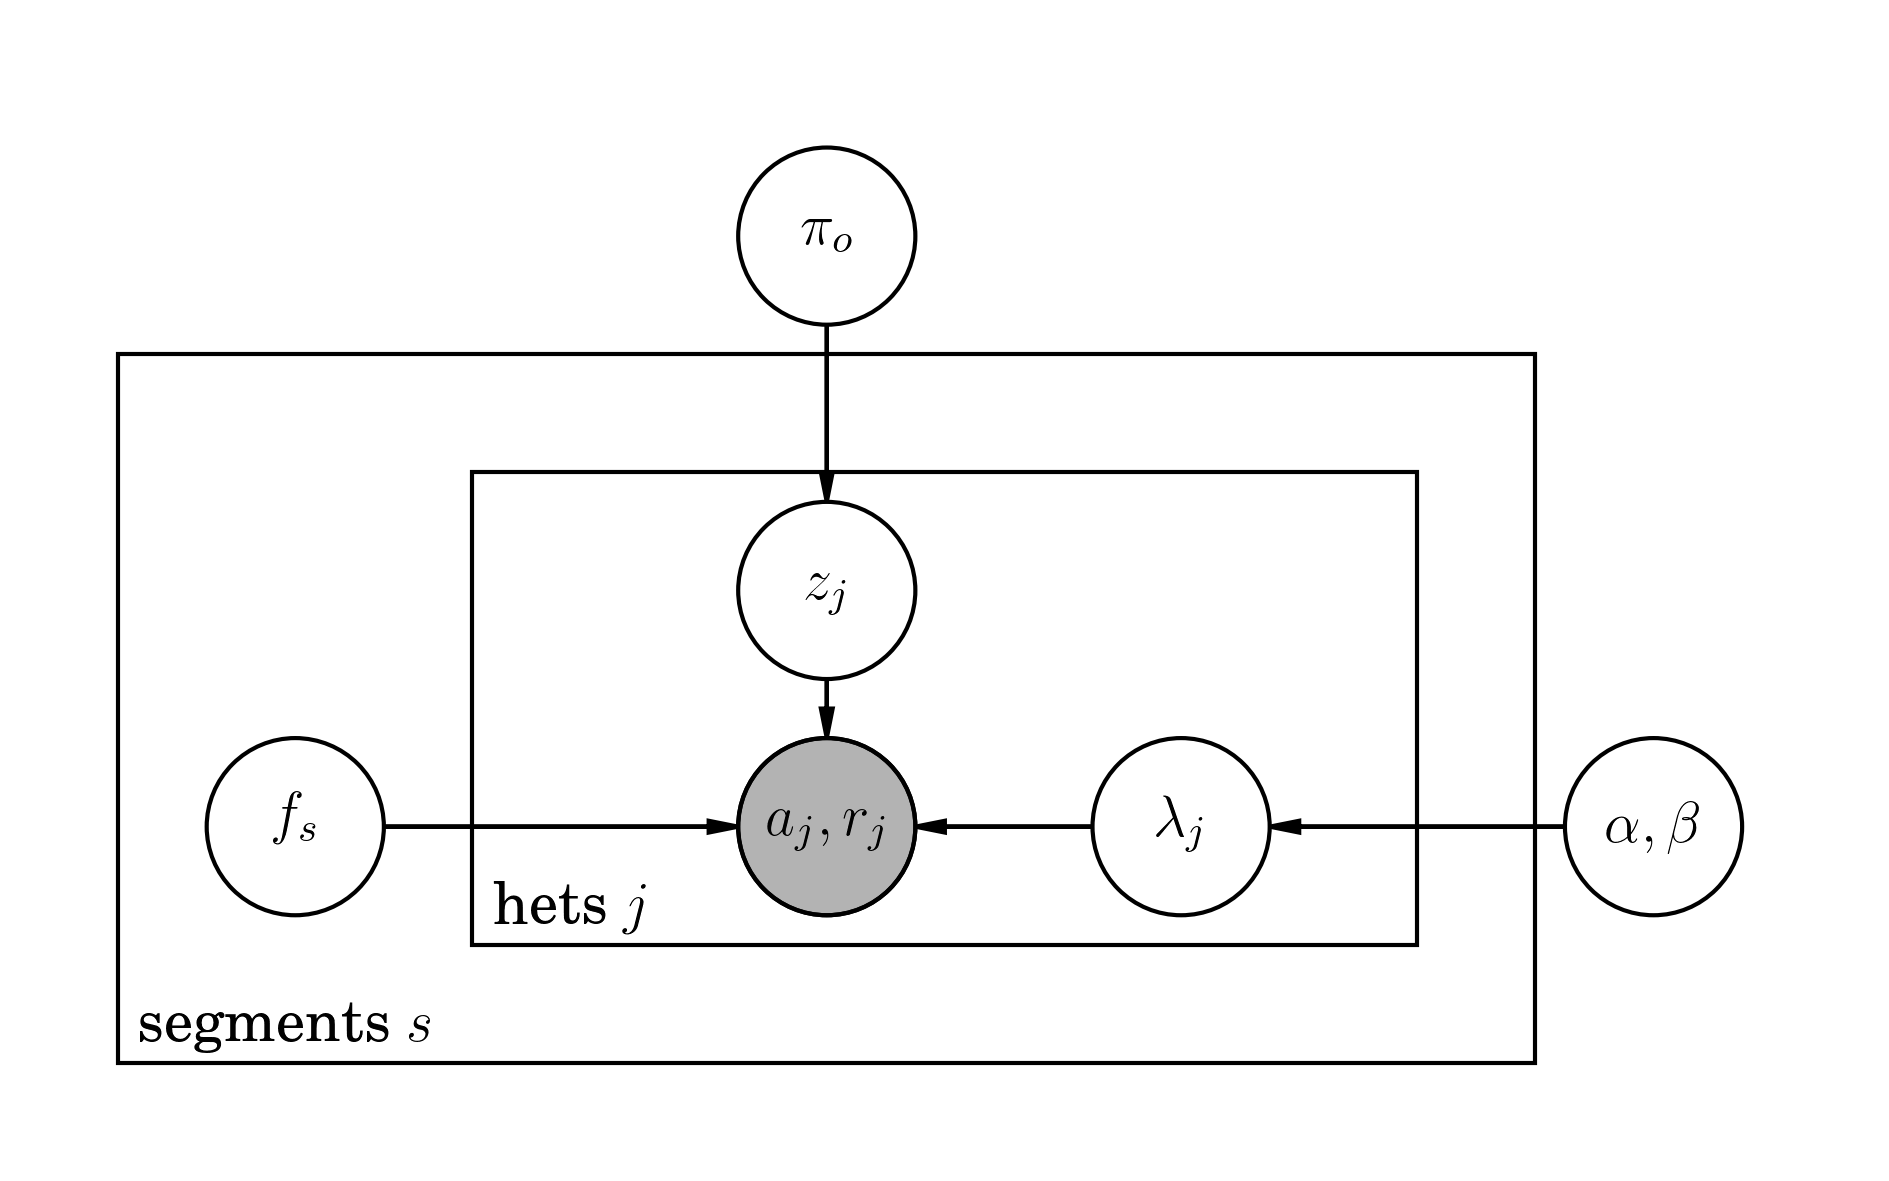
\includegraphics[width=0.8\linewidth]{ACS_model.png} 
\end{array}
$
\label{graphical_model}
\caption{Graphical model for \ACS} 
\end{figure}

As with the other parameters, we put a flat prior on ${\rm \pi}$.  Putting all the pieces together the complete-data likelihood is
\begin{equation}
P(f, a, r, z, \lambda, \alpha, \beta) = \prod_s \prod_{j \in s} P(a_j, r_j | f_s, \lambda_j, z_j) P(z_j | {\rm \pi}) P(\lambda_j | \alpha, \beta),
\end{equation}
%
where the shorthand $j \in s$ means that het site $j$ belongs to segment $s$.

We can read off the conditional probabilities necessary for Gibbs sampling from the model.  Up to constant factors the conditional on the outlier probability is,
%
\begin{align}
P(\pi_o | \{ z_j \}) \propto \pi_o^{N_{\rm o}} (1 - \pi_o)^{N - N_o},
\label{conditional_on_pi}
\end{align}
%
where $N_o = \sum_j z_{jo}$ is the number of indicator variables in the outlier state.  Thus the conditional distribution on $\pi_o$ given $\{ z_j \}$ is ${\rm Beta}(N_o, N - N_o)$.

The conditional distribution on $f_s$ is the product of likelihoods over sites $j \in s$:
%
\begin{equation}
P(f_s | a, r, \lambda, z) \propto \prod_{j \in s}
\left[ \frac{f_s^{a_j} (1 - f_s)^{r_j}}{ \left( f_s + (1-f_s) \lambda_j\right)^{n_j}} \right]^{z_{ja}}   
\left[ \frac{(1-f_s)^{a_j} f_s^{r_j} }{ \left( 1 - f_s + f_s \lambda_j\right)^{n_j}} \right]^{z_{jr}}   
\label{conditional_on_f}
\end{equation}
%
Since, in general $\lambda_j \approx 1$, this conditional approximately reduces to ${\rm Beta}(N^s_{\rm AA} + N^s_{\rm RR}, N^s_{\rm AR} + N^s_{\rm RA})$, where e.g. $N_{AR} = \sum_{j \in s} z_{ja} r_j$ is the total number of ref reads in alt minor sites.   This is the posterior distribution of the minor allele fraction given $N^s_{\rm AA} + N^s_{\rm RR}$ observations of minor alleles and $N^s_{\rm AR} + N^s_{\rm RA}$ of non-minor alleles.  Actually using this approximation would defeat the purpose of modeling the allelic bias, but it gives us a good sense of the shape of the posterior -- it is very likely to be unimodal, hence amenable to simple univariate slice sampling.

The conditional distribution on $\lambda_j$ is the product of the likelihood term for site $j$ with ${\rm Gamma}(\alpha, \beta)$.  
%
\begin{align}
P(\lambda_j | a_j, r_j, f_s, z_j) \propto & \left[  \frac{\lambda_j^{r_j}}{ \left( f_s + (1-f_s) \lambda_j \right)^{n_j}} \right]^{z_{ja}}   
\left[  \frac{\lambda_j^{r_j}}{ \left( 1 - f_s + f_s \lambda_j \right)^{n_j}} \right]^{z_{jr}}   
\lambda_j^{\alpha-1} e^{- \beta \lambda_j} \\
= &
\left( f_s + (1-f_s) \lambda_j \right)^{-n_j  (z_{ja} + z_{jr})} \lambda_j^{r_j (z_{ja} + z_{jr}) + \alpha-1} e^{- \beta \lambda_j} 
\label{conditional_on_lambda}
\end{align}
%
This conditional distribution is also easily sampled from via univariate slice sampling.

The conditional on $\beta$ is
\begin{equation}
P(\beta | \alpha, \lambda) \propto \beta^{N \alpha} e^{- \sum_j \lambda_j \beta},
\label{conditional_on_beta}
\end{equation}
which is the gamma distribution $\Gamma(N \alpha + 1, \sum_j \lambda_j)$.

The conditional on $\alpha$ is
\begin{equation}
P(\alpha | \beta, \lambda) \propto \frac{\exp \left[ \left( N \ln \beta + \sum_j \ln \lambda_j \right) \alpha \right]}{\Gamma(\alpha)^N}
\label{conditional_on_alpha}
\end{equation}
which is not of a standard form but is efficient to compute and thus amenable to univariate slice sampling.

Finally, $z_j$ is a categorical variable with priors given by ${\rm \pi}$, and its posterior can be obtained simply by plugging in its three possible values into the likelihood.

Thus we have completely specified an MCMC scheme for this model, given by Algorithm \ref{ACS_MCMC}:

\begin{algorithm}
\begin{algorithmic}[1]
\State Initialize $z_j$ to be alt minor if $a_j  < r_j$, ref minor otherwise.
\State Initialize $f_s = \left( N^s_{\rm AA} + N^s_{\rm RR} \right) / \left(N^s_{\rm AR} + N^s_{\rm RA} \right)$
\State Initialize $\lambda$ randomly and approximately equal to $1$.
\Repeat
	\State Slice sample each $f_s$  from the conditional Eq. \ref{conditional_on_f}.
	\ForAll{sites $j$}
		\State Slice sample $\lambda_j$ from the conditional Eq. \ref{conditional_on_lambda}.
		\State Sample $z_j$ from the categorical distribution defined by Eq. \ref{likelihood}.
	\EndFor
	\State Sample $\pi_o$ from the beta conditional Eq. \ref{conditional_on_pi}.
	\State Sample $\beta$ from the gamma conditional Eq. \ref{conditional_on_beta}.
	\State Slice sample $\alpha$ from the conditional Eq. \ref{conditional_on_alpha}.
\Until{convergence}
\end{algorithmic}
\caption{MCMC algorithm for \ACS}
\label{ACS_MCMC}
\end{algorithm}
\subsection{Target/SNP segment union} \label{targetsnp-segment-union}

\SL{DB can fill this in.}

\subsection{Small-segment merging} \label{small-segment-merging}

\SL{SL to update this to the new method.}

Using CBS to segment the targets in $\RCS$ results in segments that are \SL{always?} larger than $\sim$2--3 targets.  However, after taking the union of target and SNP segments, small segments with less than $\sim$2--3 targets may be introduced.  To be consistent with CBS and $\RCS$, $\ACS$ treats these small segments as spurious, and removes them by merging them with adjacent segments.

A segment is considered to be small if the number of targets it contains is strictly less than a threshold number of targets $n_t$; we take $n_t = 3$.  The small-segment merging algorithm checks each $i$th segment in turn, starting with the first, leftmost segment.  If the segment is small, it is repeatedly merged with the adjacent segment that is closer in the $L_1$ distance $|\tau_i - \tau_{i \pm 1}| + |f_i - f_{i \pm 1}|$ in copy-ratio--allele-fraction space until it is no longer small.\footnote{To be explicit, segments are reindexed after each merge, so that the new segment formed by merging segment $i$ and segment $i \pm 1$ retains the index $i$.}  Exceptions occur for adjacent segments on different chromosomes, which are never merged; in practice, this is enforced by setting the $L_1$ distance between segments on different chromosomes to be infinite.  After all segments have been checked and merged, any remaining small segments (which will be present if any chromosome contains less than $n_t$ targets) are dropped.

\subsection{Parameter optimization}\label{parameter-optimization}

\subsection{Similar-segment merging} \label{similar-segment-merging}

\subsection{Final parameter optimization} \label{final-parameter-optimization}

\section{Proposed Methods for $\texttt{hellbender}$} \label{proposed-methods-for-texttthellbender}

\subsection{Bayesian het pulldown} \label{bayesian-het-pulldown}

We are given a large data set of ref and alt read counts over many potential SNP sites and we wish to infer which sites are hets and with what probabilities.  This problem is naturally represented as a mixture model in which the hidden labels are genotypes -- hom ref, het, and hom alt.  Since the observed data are ref and alt counts is seems natural to use a binomial mixture model in which the binomial parameters are the probability of an alt read.  Then the binomial parameters are the error rate for hom ref genotypes, $1/2$ times the allelic bias for het genotypes, and $1$ minus the error rate for hom alt genotypes.  However, actual data are overdispersed because the error rate and allelic bias are random variables, not single parameters.  For example, sequencing error rates and allelic bias (for concreteness, consider mapping bias) depend on context.  Thus a beta-binomial mixture model is more appropriate.  A maximum-likelihood (MLE) approach will yield posterior probabilities on the genotypes at each locus, in particular the het probability.  It also gives the parameters of a beta distribution of allelic bias, which is useful downstream in ACS.

For generality and at no cost in complexity, consider a Dirichlet-multinomial mixture (DMM) with $K$ mixture components and $M$ classes of observed data.  For our purposes there are $K = 3$ genotypes and $M = 2$ types of read, ref and alt.  The beta-binomial distribution is the $M = 2$ case of the Dirichlet-multinomial.  The observed data are counts $n_{jm}$, the number of times class m was seen in observation $j$.  For us, each potential SNP site is a datum $j$.  Let $N_j = \sum_m n_{jm}$ denote the total read count at site $j$.  For our purposes, $\{ N_j \}$ are constants -- we are not trying to model depth of coverage here, just the proportions of the coverage allotted to ref and alt reads.

We represent hidden labels via the 1-of-$K$ encoding ${\bf z}_j = (0, 0, \ldots 1, 0, 0 \ldots)$, so $z_{jk} = 1$ when datum j comes from component $k$.  The hidden labels are multinomially distributed as $P({\bf z}_j) = {\rm Mult}({\bf z}_j | {\bf \pi})$, where $\pi_k$ is the probability of component $k$ and $\sum_k \pi_k = 1$.  Finally, the observed counts for mixture component $k$ are drawn from a Dirichlet-multinomial distribution with parameter ${\bf \alpha}_k$:

\begin{equation}
P({\bf n}_j \mid z_{jk} = 1, {\bf \alpha}_k ) = \frac{ \Gamma (A_k) }{ \Gamma (A_k + N_j) } \prod_m \frac{ \Gamma (\alpha_{km} + n_{jm}) }{ \Gamma (\alpha_{km}) },
\end{equation}
where $A_k = \sum_m \alpha_{km}$.

The EM algorithm for MLE estimates of $\{ \pi_k \}$ and $\{ \alpha_{km} \}$ requires the complete-data likelihood (CDL), that is, the joint likelihood of the observed data and hidden labels given the parameters.  In contrast, a direct approach maximizes the likelihood marginalized over the hidden variables.  The CDL of of the DMM is
\begin{align}
P({\bf z}, {\bf n} \mid {\bf \pi}, {\bf \alpha}) = & P({\bf z} \mid {\bf \pi}) P({\bf n} \mid {\bf z}, {\bf \alpha}) \\
= & \prod_{jk}  \left[ \pi_k \frac{ \Gamma (A_k) }{ \Gamma (A_k + N_j) } \prod_m \frac{ \Gamma (\alpha_{km} + n_{jm}) }{ \Gamma (\alpha_{km}) } \right]^{z_{jk}} \label{CDL}
\end{align}

In the E step of the EM algorithm, we obtain the posterior distribution on $P({\bf z} \mid {\bf n}, {\bf \pi}, {\bf \alpha})$ from Eq. (\ref{CDL}).  By inspection the posterior is a product of independent multinomials
\begin{equation}
\label{DMM_E_step}
\bar{z}_{jk} \equiv P(z_{jk} = 1 \mid {\bf n}, {\bf \pi}, {\bf \alpha})  \propto \pi_k \frac{ \Gamma (A_k) }{ \Gamma (A_k + N_j) } \prod_m \frac{ \Gamma (\alpha_{km} + n_{jm}) }{ \Gamma (\alpha_{km}) },
\end{equation}
with a normalization constant determined by the condition $\sum_k \bar{z}_{jk} = 1$.

In the M step of the EM algorithm we take the expectation of the log-CDL with respect to the posterior on ${\bf z}$ and maximize with respect to ${\bf \pi}$ and ${\bf \alpha}$.  That is, we maximize
\begin{equation}
\sum_{jk}  \bar{z}_{jk} \left\{ \log \pi_k + \log \frac{\Gamma (A_k)}{ \Gamma (A_k + N_j)}  + \sum_m \log \frac{ \Gamma (\alpha_{km} + n_{jm})}{\Gamma (\alpha_{km})}  \right\}.
\end{equation}

Maximizing with respect to $\pi_k$ with a Lagrange multiplier for the constraint $\sum_k \pi_k = 1$
\begin{equation}
\label{DMM_M_step_pi}
\pi_k = \frac{ \sum_j \bar{z}_{jk} }{\sum_{j \ell} \bar{z}_{j \ell}}
\end{equation}

To maximize with respect to ${\bf \alpha}$ we use the fact that if we are trying to maximize $f({\bf x})$ and have a current guess of ${{\bf x}_0}$, then an improved guess may be obtained by maximizing $g({\bf x})$, where $g({\bf x}_0) = f({\bf x}_0)$ and $g({\bf x}) \le f({\bf x})$ for all ${\bf x}$.  Furthermore, repeating this gives an iterative optimization that converges to a local maximum.  Using bounds (\ref{bound1}) and (\ref{bound2}) and dropping additive constants, we find that the iterative step is to maximize the lower bound
\begin{equation}
\sum_{jk}  \bar{z}_{jk} \left\{ - \left( \psi(\hat{A}_k + N_j) - \psi(\hat{A}_k) \right) A_k + \sum_m \hat{\alpha}_{km}  \left( \psi(\hat{\alpha}_{km}  + n_{jm}) - \psi(\hat{\alpha}_{km}) \right)  \log(\alpha_{km} )   \right\}.
\end{equation}
with respect to $\alpha_{km}$ treating the ``old'' guesses $\hat{\alpha}_{km}$ as constants.  This maximization is a straightforward matter of setting the derivative to zero and gives the fixed-point iteration
\begin{equation}
\label{DMMiteration}
\alpha_{km} = \hat{\alpha}_{km} \frac{\sum_j \bar{z}_{jk}  \left( \psi(\hat{\alpha}_{km}  + n_{jm}) - \psi(\hat{\alpha}_{km}) \right)} {\sum_j \bar{z}_{jk} \left( \psi(\hat{A}_k + N_j) - \psi(\hat{A}_k) \right)}
\end{equation}

As is often the case with mixture models, we risk converging to a bad local maximum if parameters are initialized poorly.  Following the approach used by Thomas Minka in his FastFit software, we obtain a good initial guess by fitting a Dirichlet mixture model (as opposed to a Dirichlet-multinomial model) on effective multinomial pseudodata.  That is, instead of working with \textit{counts} $n_{jm}$, work with \textit{proportions} $p_{jm} = n_{jm} / N_j$.  Since $\sum_m p_{jm} = 1$, ${\bf p}_j$ can be interpreted as a multinomial distribution drawn from a Dirichlet mixture.  This preprocessing step maps the original count data onto the $(M-1)$-dimensional simplex, and we can then assign the pseudo-multinomials $\{ {\bf p}_j \}$ to $K$ clusters via the $K$-means algorithm.  Define the indicator variable $\chi_{jk} = 1$ if pseudo-multinomial ${\bf p}_j$ is assigned to cluster $k$ and let $\chi_{jk} = 0$ otherwise.

We initialize $\pi_k$ as the empirical proportion of mixture component $k$ in the clustering step.  That is
\begin{equation}
\label{DMM_initialize_pi}
\pi_k = \frac{\sum_j \chi_{jk}}{N} = \frac{N_k}{N}
\end{equation}
where $N_k$ is the number of pseudo-multinomials assigned to cluster $k$.

Then for each component $k$ we initialize the Dirichlet parameter vector ${\bf \alpha_k}$ via moment matching.  Parameterize ${\bf \alpha_k}$ as ${\bf \alpha}_k = s_k {\bf \theta}_k$, where $\sum_m \theta_{km} = 1$ is the mean of the Dirichlet distribution and $s$ is its concentration.  Since multinomials $S_k = \{ {\bf p}_j \, : \, \chi_{jk} = 1 \}$ are presumed drawn from Dirichlet distribution with parameter ${\bf \alpha}_k$, we set the theoretical mean ${\bf \theta}_k$ to the empirical mean of $S_k$:
\begin{equation}
\theta_{km} = \left\langle   {\bf p}_j \in S_k \right\rangle = \frac{1}{N_k} \sum_j \chi_{jk} p_{jm}
\label{1st_moment_matching}
\end{equation}

Moment matching of the $m$-th diagonal component of the covariance gives
\begin{align}
\frac{ \alpha_{km} \left( \sum_\ell \alpha_{k \ell} - \alpha_{km} \right) }{\left( \sum_\ell \alpha_{k \ell}\right)^2 \left( \sum_\ell \alpha_{k \ell} + 1 \right) }=& {\rm cov}(S_k)_{mm} =  \left\langle   p_{jm}^2 \in S_k \right\rangle - \left\langle   p_{jm} \in S_k \right\rangle^2 \\
%
\frac{ \theta_{km} (1 - \theta_{km})} {s_k + 1} =& \frac{1}{N_k} \sum_j \chi_{jk} p^2_{jm} \\
s_k = & \frac{  \theta_{km} - \frac{1}{N_k} \sum_j \chi_{jk} p^2_{jm}}{\frac{1}{N_k} \sum_j \chi_{jk} p^2_{jm} - \theta_{km}^2 }
\label{2nd_moment_matching}
\end{align}

Since these $M$ estimates $s_k$ do not need to agree, we simply take their average.


The EM algorithm for DMM inference is summarized in Algorithm \ref{DMM}.

\begin{algorithm}
\begin{algorithmic}[1]
\State Form pseudo-multinomial data $p_{jm} = n_{jm} / N_j$
\State Find $K$ clusters of this pseudodata via the $K$-means algorithm.
\State Initialize ${\bf \pi}$ via Eq. \ref{DMM_initialize_pi}
\State Initialize $\{ \alpha_{km} \}$ via Eqs. \ref{1st_moment_matching} and \ref{2nd_moment_matching}
\Repeat
	\State Update $\bar{z}_{jk}$ via Eq. \ref{DMM_E_step}
	\State Update ${ \bf \pi}$ via Eq. \ref{DMM_M_step_pi}
		\Repeat
		\State update $ \{ \alpha_{km} \}$ via Eq. \ref{DMMiteration}
	\Until{convergence}
\Until{convergence}
\end{algorithmic}
\caption{EM algorithm for Dirichlet-multinomial mixture model}
\label{DMM}
\end{algorithm}

Returning to our original task, we obtain three mixture components with Dirichlet parameters $(\alpha_{k1}, \alpha_{k2})$.  The mean proportion of alt reads (WLOG we choose $m = 1$ to be alt and $m=2$ to be ref) are $\alpha_{k1}/(\alpha_{k1} + \alpha_{k2})$, so we can assign mixture labels $k = 1, 2, 3$ to genotypes by comparing these proportions to $0$ (hom ref), $1/2$ (het) and $1$ (hom alt). The posterior probability $\bar{z}_{jk}$ is the probability that site $j$ has genotype $k$, which is exactly what we need for a probabilistic het pulldown.

\subsection{Improving \ACS ~model sampling} \label{ACS_aux_variable}
The \ACS model likelihood has thorny factors of the form $\left( f_s + (1 - f_s) \lambda_j \right)^{-n_j}$ (and `` $f \leftrightarrow 1 - f$ '').  Other than these, everything comes from exponential family distributions, is log-concave etc.  If we could rid ourselves of this term and replace it with a standard distribution we could greatly speed our Gibbs sampling.  Consider the identities
%
\begin{align}
\left( f_s + (1 - f_s) \lambda_j \right)^{-n_j} =& \frac{1}{\Gamma(n_j)} \int_0^\infty w_j^{n_j - 1} e^{-\left( f_s + (1 - f_s) \lambda_j \right) w_j} \, dw_j \\
\left( 1 - f_s + f_s \lambda_j \right)^{-n_j} =& \frac{1}{\Gamma(n_j)} \int_0^\infty w_j^{n_j - 1} e^{-\left(1 -  f_s + f_s \lambda_j \right) w_j} \, dw_j \\
1 = & \frac{1}{\Gamma(n_j)} \int_0^\infty w_j^{n_j - 1} e^{-w_j} \, dw_j
\end{align}
%
Applying these to the likelihood terms when $z_{ja} = 1$, $z_{zr} = 1$, and $z_{jo} = 1$ respectively we see that if we augment the state space with an auxiliary variable $w_j$ for each het site we may replace the likelihood Eq. \ref{likelihood} with the more tractable
\begin{equation}
P(a_j, r_j | f_s, \lambda_j, w_j, z_j) \propto w_j^{n_j - 1}
\left[ f_s^{a_j} (1 - f_s)^{r_j} \lambda_j^{r_j}  e^{-\left( f_s + (1-f_s) \lambda_j \right)w_j} \right]^{z_{ja}}   
\left[ (1-f_s)^{a_j} f_s^{r_j} \lambda_j^{r_j} e^{-\left( 1 - f_s + f_s \lambda_j \right)w_j} \right]^{z_{jr}}   
\left[ \frac{a_j! r_j!}{(n_j + 1)!} e^{-w_j}\right]^{z_{jo}}
\label{augmented_likelihood}
\end{equation}
%
The complete-data likelihood becomes
\begin{equation}
P(f, a, r, z, \lambda, w, \alpha, \beta) = \prod_s \prod_{j \in s} P(a_j, r_j | f_s, \lambda_j, w_j,  z_j) P(z_j | {\rm \pi}) P(\lambda_j | \alpha, \beta),
\end{equation}
%
with the terms $P(z_j | {\rm \pi})$ and $P(\lambda_j | \alpha, \beta)$ unchanged from above.  The virtues of this ``de-marginalization'' are apparent when we consider conditional probabilities.  The conditional on $w_j$ is
%
\begin{equation}
P(w_j | a_j, r_j, f_s, \lambda_j, z_j) \propto w_j^{n_j - 1} e^{- \left[ \left( f_s + (1-f_s) \lambda_j \right) z_{ja} + \left( 1 - f_s + f_s \lambda_j \right) z_{jr} + z_{jo} \right] w_j},
\label{augmented_conditional_on_w}
\end{equation}
%
which is a gamma distribution.  The conditional on $\lambda_j$ is
%
\begin{equation}
\lambda_j^{ (z_{ja} + z_{jr})r_j + \alpha - 1} e^{-\left[ (1-f_s) w_j z_{ja} + f_s w_j z_{jr} + \beta \right] \lambda_j},
\label{augmented_conditional_on_lambda}
\end{equation}
another gamma distribution.  The conditional on $f_s$ is
%
\begin{equation}
P(f_s | a, r, \lambda, w, z) = f_s^{\sum_{j \in s} (a_j z_{ja} + r_j z_{jr})}  (1-f_s)^{\sum_{j \in s} (a_j z_{jr} + r_j z_{ja})} e^{ \sum_{j \in s} (\lambda_j w_j - 1) (z_{ja} - z_{jr})f_s}.
\label{augmented_conditional_on_f}
\end{equation}
%
Although this is not a standard distribution, it is the product of only three factors, as opposed to one factor for each $j \in s$, a great improvement.  Furthermore, it is of the form $f^a (1-f)^b e^{c f}$.  It turns out that functions of this form on $[0,1]$ can be approximated extremely well by a beta distribution\footnote{I have an interactive SAGE notebook verifying this claim for a wide range of parameters, but now that I know it empirically to be true an analytic proof shouldn't be too hard.} proportional to $f^\sigma (1-f)^\tau$.  Thus if we use this beta distribution as a proposal distribution for Metropolis-Hastings sampling of the conditional Eq. \ref{augmented_conditional_on_f} we will obtain essentially perfect, uncorrelated samples with a single step.  That is, we can achieve the ideal state of Gibbs sampling.  To obtain the desired approximation, we match first and second derivatives of the log-conditional with the log of the beta approximation at the mode of the log-conditional.  This can all be done analytically.  The mode $f_0$ is given by
%
\begin{equation}
f_0 = \frac{-(a+b) + c + \sqrt{(a+b)^2 + 2(a-b)c + c^2} }{2c}
\end{equation}
%
and the result of matching derivatives is
\begin{equation}
\sigma = a + c f_0^2, \, \tau = -c f_0^2 + 2 c f_0 + b - c.
\end{equation}
%
The higher-level parameters $\alpha$, $\beta$, and $\pi_o$, and the indicators $z_j$ are unaffected by this change and are sampled as before.  To summarize what we have accomplished by adding auxiliary variables, we now have perfect, uncorrelated draws from the conditional distribution of every variable using standard distributions (beta, gamma, categorical), the parameters of which are obtained from simple arithmetic.  The only exception is $\alpha$, which we must still slice-sample, but that only occurs once per Gibbs sweep.  The computational savings ought to be enormous.

\subsection{Model-comparison test for segment merging} \label{likelihood-based-segment-merging}

\SL{I'll fill this in once it's worked out.}

%%%APPENDICES
\appendix

\section{Finding Tight Lower Bounds on Convex and Non-convex Functions} \label{bounds}

Given a function $f(x)$ and an arbitrary value $x_0$, we seek a lower bound $g(x) \le f(x)$ that is tight at $x_0$, that is, $g(x_0) = f(x_0)$.  If $f(x)$ is convex, that is, if $f^\prime(x)$ is non-decreasing, the linearization $g(x) = f(x_0) + f^\prime(x_0)(x-x_0)$ is such a bound.  More generally, suppose $h(x) f^\prime(x)$ is non-decreasing.  Instead of approximating $f^\prime(x) \approx f^\prime(x_0)$, perhaps we can approximate $h(x) f^\prime(x) \approx h(x_0) f^\prime(x_0)$ via a candidate lower bound $g(x)$ for which

\begin{align}
g^\prime(x) =& \frac{ h(x_0) f^\prime(x_0) } {h(x)} \\
g(x) =& f(x_0) + h(x_0) f^\prime(x_0)  \int_{x_0}^x \frac{d t}{h(t)}
\end{align}

\begin{lemma}
Such a function $g(x)$ is a tight lower bound on $f(x)$ if $h(x) f^\prime(x)$ is non-decreasing for some non-negative function $h(x)$.
\end{lemma}

\begin{proof}
By the Fundamental Theorem of Calculus,

\begin{align}
f(x) - g(x) =& \int_{x_0}^{x} \left( f^\prime(t) - g^\prime(t) \right) \, dt \\
=&  \int_{x_0}^{x} \frac{ h(t) f^\prime(t) - h(x_0) f^\prime(x_0) } {h(t)} \, dt
\end{align}

By the monotonicity of $h(x)$, the integral is non-positive for $x > x_0$ and non-negative for $x < x_0$.  Either way, the resulting integral is negative, so $g(x) \le f(x)$.
\end{proof}

For Dirichlet-multinomial inference, we use the special case $h(x) = x$.

\begin{corollary} 
If $x f^\prime(x)$ is non-decreasing for $x > 0$ then for any $x_0 > 0$
\begin{equation}
f(x) \ge f(x_0) + x_0 f^\prime(x_0) \left( \log(x) - \log(x_0) \right)
\end{equation}
\end{corollary}


Two important cases are $f_1(x) = \log \Gamma(x) / \Gamma(x + n)$ and $f_2(x) = \log \Gamma(x + n) / \Gamma(x) = -f_1(x)$, where $n$ is a whole number.  Using the recursive identity $\Gamma(n+1) = n \Gamma(n)$ we have

\begin{equation}
f_1(x) = -\sum_{k=0}^{n-1} \log(x + k), \quad f^\prime_1(x) = -\sum_{k=0}^{n-1} \frac{1}{x+k}, \quad f_1^{\prime \prime}(x) = \sum_{k=0}^{n-1} \frac{1}{(x+k)^2}
\end{equation}

from which we see that $f_1(x)$ is convex and the usual linearization bound holds

\begin{align} \label{bound1}
\log \frac{ \Gamma(x) }{ \Gamma(x + n) } \ge & \log \frac{ \Gamma(x_0) }{ \Gamma(x_0 + n) } - \left( \psi(x_0 + n) - \psi(x_0) \right) (x - x_0)
\end{align}

where $\psi(x) = \frac{d}{dx} \log \Gamma(x)$ is the digamma function.  As for $f_2(x) = - f_1(x)$, it is not convex, but

\begin{equation}
x f_2^\prime(x) = \sum_{k=0}^{n-1} \frac{x}{x+k} = \sum_{k=0}^{n-1} \frac{1}{1+k/x},
\end{equation}

which is increasing since each denominator is decreasing.  Thus we apply the above corollary to obtain

\begin{equation} \label{bound2}
\log \frac{ \Gamma(x + n) }{ \Gamma(x) } \ge \log \frac{ \Gamma(x_0 + n) }{ \Gamma(x_0) } + x_0 \left( \psi(x_0 + n) - \psi(x_0) \right)  \left( \log(x) - \log(x_0) \right)
\end{equation}
\end{document}
